\documentclass{article}
\usepackage{graphicx} % Required for inserting images
\usepackage{enumerate}
\usepackage{amssymb}
\usepackage[a4paper, total={6in, 8in}]{geometry}
\usepackage{hyperref}
\usepackage{amsmath}
\usepackage{amsthm}
\usepackage{cancel}

\usepackage{lastpage}
\usepackage{fancyhdr}
\usepackage{geometry}
\geometry{margin=1in}
\usepackage{underscore}
\usepackage{subcaption}
\usepackage{fancyvrb}
\usepackage{listings}
\lstset{basicstyle=\small\ttfamily, columns=flexible, breaklines=true}
\usepackage{tabularx}
\usepackage{float}
\usepackage{makecell}

\usepackage{mdframed}
\usepackage{lipsum}

\usepackage{hyperref}
\usepackage{multicol}
\usepackage{fancyhdr}
\pagestyle{fancy}
\fancyhf{} % Clear default headers and footers

% Add a simple header
\fancyhead[L]{\textbf{CSE-103 Notes}} % Left-aligned header text
\fancyhead[R]{\textbf{Spring 2025}}   % Right-aligned header text

% Add page numbers in the footer
\fancyfoot[C]{\thepage\ of \pageref{LastPage}} % Center-aligned footer with total pages

% Disable red box around page numbers (using hyperref)
\usepackage{hyperref}
\hypersetup{
    colorlinks=false, % Enable colored links
    linkcolor=blue,  % Set the color of internal links (like page numbers)
    urlcolor=blue,   % Set the color of URLs
    pdfborder={0 0 0} % Remove the border around links
}

\usepackage{tikz,tcolorbox}
\usepackage{xcolor}
 

\title{CSE-103: Computational Models\\ Lecture Notes}
\author{Mann Malviya}
\date{Spring 2025}

\begin{document}
\maketitle
\maketitle
\tableofcontents
\newpage

\section*{Introduction}
\addcontentsline{toc}{section}{Introduction} 


\subsection*{Textbooks}
\addcontentsline{toc}{subsection}{Textbooks} 

\begin{enumerate}
    \item Introduction to the Theory of Computation by Michael Sipser
    \begin{figure}[H]
        \centering
        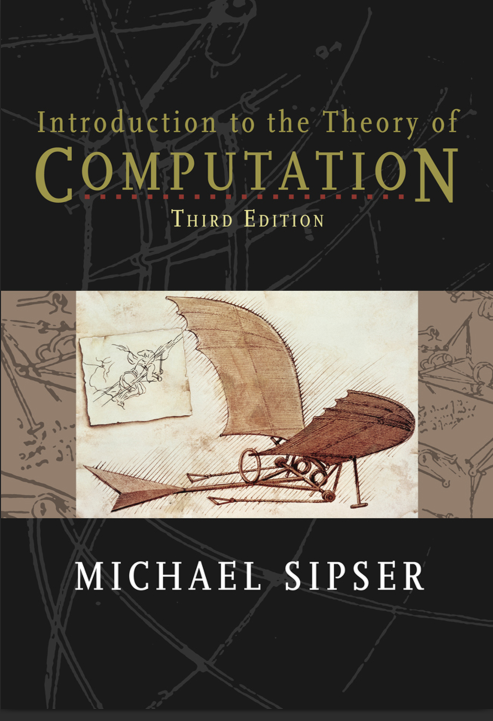
\includegraphics[scale=2]{103_TB.png}
        \caption*{\centering{Introduction to the Theory of Computation \\by Michael Sipser}}
    \end{figure}
\end{enumerate}

\begin{center}
	\rule{450pt}{1pt} 
\end{center}

\subsection*{What is this Doc?}
\addcontentsline{toc}{subsection}{What is this Doc?}
This document shall contain my notes for the class CSE-103: Computational Models offered at UCSC, taught by Assistant Prof. Daniel Fremont. This document will contain notes from the lectures(possibly verbatim?) and may contain some additional information, either from the text or other sources that I find useful.


\begin{center}
	\rule{450pt}{3pt} 
\end{center}
\newpage



\section*{Lecture 1}
\addcontentsline{toc}{section}{Lecture 1}

\subsection*{Overview of the Course}
\addcontentsline{toc}{subsection}{Overview of the Course}




\subsection*{Learning Objectives}
\addcontentsline{toc}{subsection}{Learning Objectives}
After taking this course, you will be able to:
\begin{enumerate}
    \item Interpret and design finite automata (DFAs and NFAs) and regular expressions.
    \item Interpret and design context-free grammars (CFGs) and pushdown automata.
    \item Prove basic properties of regular and context-free languages.
    \item Interpret and design Turing machines(TMs).
    \item Prove basic languages are decidable or Turing-recognizable.
    \item Construct reductions between problems and apply such reductions to establish undecidability of problems
    \item Construct polynomial-time algorithms/verifiers and polynomial-time reductions and use them to show languages are in P, NP, or are NP-complete.
\end{enumerate}


\subsection*{Outline of the Course}
\addcontentsline{toc}{subsection}{Outline of the Course}

\begin{center}
	\rule{450pt}{1pt} 
\end{center}
\newpage

\section*{Lecture 2:}


\end{document}